\documentclass[solution,addpoints,12pt]{exam}
\usepackage{amsmath}
\usepackage{amsthm}
\usepackage{amssymb}
\usepackage{tikz}
\usepackage{animate}
\usepackage{hyperref}
\usepackage{booktabs}
\newtheorem{theorem}{Theorem}
\newtheorem{lemma}[theorem]{Lemma}

\newenvironment{Solution}{\begin{EnvFullwidth}\begin{solution}}{\end{solution}\end{EnvFullwidth}}

\printanswers
%\unframedsolutions
\pagestyle{headandfoot}

%%%%%%%%%%%%%%%%%%%%%%%%%%%%%%%%%%%%%%%%%%%%%%%%%%%%%%
%%%%%%%%%%%%%%%%%%% INSTRUCTIONS %%%%%%%%%%%%%%%%%%%%%
% * Fill in your name and roll number below

% * Answer in place (after each question)

% * Use \begin{solution} and \end{solution} to typeset
%   your answers.
%%%%%%%%%%%%%%%%%%%%%%%%%%%%%%%%%%%%%%%%%%%%%%%%%%%%%%
%%%%%%%%%%%%%%%%%%%%%%%%%%%%%%%%%%%%%%%%%%%%%%%%%%%%%%

% Fill in the details below
\def\studentName{\textbf{Name:\hspace{15mm}}}
\def\studentRoll{\textbf{Roll No:\hspace{15mm}}}

\firstpageheader{CS 7015 - Deep Learning - Assignment 1}{}{\studentName, \studentRoll}
\firstpageheadrule

\newcommand{\brac}[1]{\left[ #1 \right]}
\newcommand{\curly}[1]{\left\{ #1 \right\}}
\newcommand{\paren}[1]{\left( #1 \right)}
\newcommand{\card}[1]{\left\lvert #1 \right\rvert}

\begin{document}
\textbf{Instructions:}
\begin{itemize}
    \itemsep0em
    \item This assignment is meant to help you grok certain concepts we will use in the course. Please don't copy solutions from any sources.
    \item Avoid verbosity.
    \item The assignment needs to be written in latex using the attached tex file. The solution for each question should be written in the solution block in space already provided in the tex file. \textbf{Handwritten assignments will not be accepted.}
    
\end{itemize}

\begin{questions}

\question \textbf{Partial Derivatives}
          \newline
          \begin{parts}
   

        \part Find the derivative of $g(\rho)$ with respect to $\rho$ where $g(\rho)$ is given by,
      \[ g(\rho) = \frac{1}{2} \rho log\frac{\rho}{\rho+\hat{\rho}} + \frac{1}{2} \hat{\rho} log\frac{\hat{\rho}}{\rho+\hat{\rho}} \]
      (You can consider $\hat{\rho}$ as constant)
      \begin{solution}
      \vspace*{50mm}
      \end{solution}
            \part Consider the following computation ,
                  \begin{center}
                  \hspace*{-15mm}
                    \tikzstyle{neuron1}=[circle,draw=blue!50,fill=blue!20,thick,minimum size=1mm]
                    \tikzstyle{neuron2}=[circle,draw=blue!50,fill=blue!20,thick,minimum size=6mm]
                    \tikzstyle{input}=[circle,draw=black!50,fill=black!20,thick,minimum size=6mm]
                    \begin{tikzpicture}
                        \node [neuron1] (neuron1) at (0.1,6)  {$\frac{1 + tanh(wx+b)}{2}$} ;
                        \node [neuron2] (neuron2) at (4,6)  {$sigm(z)$} ;
                        \node (input1) at (-3,6)  {$x$};
                        \node (input0) at (-3,5)  {$1$};
                        \node (output0) at (6,6)  {$f(x)$};
                        \node (formula) at (0,4) {where $ z = \frac{1 + tanh(wx+b)}{2}$ and $f(x) = sigm(z)$};
                        \node (formula2) at (0,3) {by definition : $sigm(z) = \frac{1}{1+e^{-z}}$ and $tanh(z) = \frac{e^{z} - e^{-z}}{e^{z} + e^{-z}} $ };
                        \draw [->] (input0) -- (neuron1);
                        \draw [->] (input1) -- (neuron1);
                        \draw[->] (neuron1) -- (neuron2);
                        \draw [->] (neuron2) -- (output0);
                        \node (label) at (2.3,6.3) {$z$};
                    \end{tikzpicture}
                  \end{center}
                  The value $L$ is given by, 
                  \[ 
                     L = - y \log (f(x))          \]
                  Here, $x$ and $y$ are constants and $w$ and $b$ are parameters that can be modified.
                  In other words, $L$ is a function of $w$ and $b$.

                  Derive the partial derivatives, $\frac{\partial L}{\partial w}$ and $\frac{\partial L}{\partial b}$.
   
              \begin{solution}
                \vspace*{100mm}
                
              \end{solution}

         \end{parts}  
         

\question 
\textbf{Chain Rule}:
    \begin{parts}
            \part Consider the evaluation of $E$ as given below,
                  \[
                    E = h(u,v,w,x) = 2*f(au + bv) - g(cw + dx))
                  \]
                  \begin{minipage}{0.45\linewidth}
                  Represented as graph:\\
                  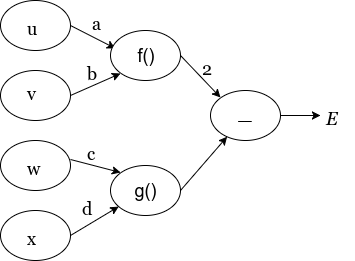
\includegraphics[scale=0.5]{download.png}
                  \end{minipage}\quad
                  \begin{minipage}{0.55\linewidth}
                  Here $u,v,w,x$ are inputs (constants) and $a,b,c,d$ are parameters (variables). $f$ and $g$ are the activation functions (with $z$ as input) defined as below:
                  \begin{eqnarray*}
                  f(z) = sigm(z) \qquad \qquad g(z) = tanh(z)
                  \end{eqnarray*}
                  \end{minipage}\\                  
                  Note that here $E$ is a function of parameters $a,b,c,d$.
                  Compute the partial derivatives of $E$ with respect to the parameters $a$, $b$, $c$ and $d$ \textit{i.e.} $\frac{\partial E}{\partial a}$, $\frac{\partial E}{\partial b}$, $\frac{\partial E}{\partial c}$ and $\frac{\partial E}{\partial d}$.
                  \begin{solution}
                  \vspace*{80mm}
                  \end{solution}
            \part Assume that $z = f(x, y)$, where $x = uv$ and $y = \frac{u}{v}$. We use $f_{x}$ to denote the partial derivative $\frac{\partial f}{\partial x}$. Using the chain rule, express  $\frac{\partial z }{\partial u}$ and  $\frac{\partial z }{\partial v}$ in terms of $u$, $v$, $f_{x}$ and $f_{y}$. 
        \begin{solution}
            \vspace*{20mm}
        \end{solution}
            
    
    \part Given the change of variables as mentioned in the previous part: $x = uv$ and $y = \frac{u}{v}$, calculate the Jacobian of this transformation.
    \begin{solution}
    \vspace*{20mm}
    \end{solution}
    \part Calculate the Jacobian of the transformation for rectangular coordinates; \textit{i.e.}, the Jacobian of $x$ = $r sin \theta$, $y$ = $r cos \theta$, $z$ = $z$, (hint: using the relevant partial derivatives)
    \begin{solution}
    \vspace*{20mm}
    \end{solution}
    \end{parts}
\question  \textbf{Visit Taylor Series} The first order derivative of a function $f$ is defined by the following limit,
          \begin{equation} \label{eq:deriv_definition}
            \frac{df(x)}{dx} = \lim_{h \to 0} \frac{f(x + h) - f(x)}{h}
          \end{equation}
          On observing the above definition we see that the derivative of a function is the ratio of
          change in the function value to the change in the function input, 
          when we change the input by a small quantity (infinitesimally small).
          A first degree approximation based on eq. \ref{eq:deriv_definition} would be the following.
          \begin{equation}
            f(x+h) \approx f(x) + h \frac{df(x)}{dx}
          \end{equation}
          Consider $f(x) = ln(x+5)$. 
         \begin{parts}
         \part
          Estimate the value of $f(1)$,$f(1.1)$ and $f(2.5)$ using the above formula.
                \begin{solution}
                \vspace*{5mm}
                \end{solution}
          \part Compare these estimates to the actual values of function $f(1)$,$f(1.1)$ and $f(2.5)$. Explain the discrepancy as we increase the value.
                \begin{solution}
                \vspace*{10mm}
                \end{solution}
          \part Can we get a better estimate of $f(1)$,$f(1.1)$ and $f(2.5)$ ? How?
                \begin{solution}
                \vspace*{20mm}
                \end{solution}
            
        \part Consider $g(x) = a + be^{x} + c*\cos(x)$. Find a, b, c $\in$ R such that $g$ approximates $f$ at
$x$ = 0. (i.e. by matching the (i) direct values (ii) first derivative and (iii) second derivative at $x = 0$).
        \begin{solution}
        \vspace*{70mm}
        \end{solution}
          
\end{parts}

\question
\textbf{Differentiation of function of multiple variables}
          \begin{equation*}
            \begin{aligned}
              s_1 & = tan(w_1 x) \\
              s_2 & = sec(w_2 x + s_1) \\
              s_3 & = sin(w_3 s_1 + w_4 s_2) \\
              s_4 & = cos(w_5 s_3 + w_6) \\
              y   & = tanh(w_7 s_4 + w_8)
            \end{aligned}
          \end{equation*}

          An alternative representation of the function $y$ is given in the figure below.
          \begin{center}
            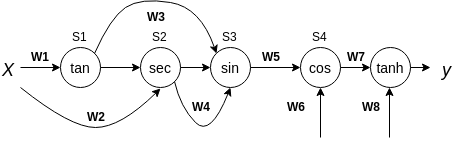
\includegraphics[scale=0.7]{fig2.png}
          \end{center}

          Compute the derivatives $\frac{dy}{dw_1}$ and $\frac{dy}{dw_2}$ (show all the steps).

          \begin{solution}
          \vspace*{70mm}
          \end{solution}
          
\question \textbf{Differentiation of vectors/matrices}
          \newline
          Consider vectors $\boldsymbol{u,b} \in \mathbb{R}^d$, and matrix $\boldsymbol{A} \in \mathbb{R}^{n \times n}$.
          \newline
          The derivative of a scalar $f$ w.r.t. a vector $\boldsymbol{u}$ is a vector by itself, given by
          \[
            \nabla f = \left( \frac{\partial f}{\partial u_1}, \frac{\partial f}{\partial u_2}, \dots, 
                         \frac{\partial f}{\partial u_n} 
                       \right)
          \]
          \newline
         ( \textbf{Hint}:  The derivative of a scalar $f$ w.r.t. a matrix $\boldsymbol{X}$, is a matrix whose $(i,j)$ component is $\frac{\partial f}{\partial X_{ij}}$, where $X_{ij}$ is the $(i,j)$ component of the matrix $\boldsymbol{X}$.)
         \newline
         \begin{parts}
         \part Derive the expression for the derivative:  $ \nabla \textbf{\textit{u}}^{T}\textbf{\textit{Au}} + \textbf{\textit{b}}^{T}\textbf{\textit{u}}$.
         \begin{solution}
         \vspace*{20mm}
         \end{solution}
         \part Compare your results with derivatives for the scalar equivalents
          of the above expressions $au^{2}+ bu$.
         \begin{solution}
         \vspace*{20mm}
         \end{solution}
         \part Derive the Hessian: $\frac{\partial^{2}f}{\partial \textbf{u}\partial \textbf{u}^{T}}$ given that $f = \textbf{\textit{u}}^{T}\textbf{\textit{Au}} + \textbf{\textit{b}}^{T}\textbf{\textit{u}}$
         \begin{solution}
         \vspace*{20mm}
         \end{solution}
         
         \end{parts}
\question \textbf{Encoding Tongue Twister :} You have been assigned a task to encode a tongue-twister
phrase compactly:
`clean clams crammed in clean clans'.
For convenience, you are given the frequency distribution as below.
\begin{table*}[h]
    \centering
    \begin{tabular}{c|c}
        \toprule
         Char & Frequency  \\
         \midrule
         a & 5\\
         c & 5 \\
         d & 1 \\
         i & 3 \\
         l & 4 \\
         m & 3 \\
         n & 4 \\
         r & 1 \\
         s & 2 \\
         space & 5\\
         \bottomrule
    \end{tabular}
    \label{tab1}
\end{table*}
\begin{parts}
\part One way to encode this sequence is to use fixed length code with each code word long enough to encode ten different symbols. How many
bits
would
be
needed
for
this
33-character
phrase
using
such
a
fixed-length
code?
\begin{solution}
\vspace*{10mm}
\end{solution}
\part What are the
minimum
number
of
bits
needed (theoretically)
to
encode
the
entire
phrase
,
assuming
that
each
character
is
independent
of
the
surrounding
character? 
Hint: We can calculate the average information (in other words, bits needed) of a symbol using entropy information.
\begin{solution}
\vspace*{50mm}
\end{solution}
\end{parts}
\question \textbf{Plotting Functions for Great Good}
          \begin{parts}
            \part Consider the variable $x$ and functions $h_{11}(x)$, $h_{12}(x)$ and $h_{21}(x)$ such that

                  \begin{align*}
                    h_{11}(x) = \frac{1}{1 + e^{-(500 x + 30)}}  \\
                    h_{12}(x) = \frac{1}{1 + e^{-(500 x - 30)}}  \\
                    h_{21} = h_{11}(x) - h_{12}(x)  \\
                  \end{align*}
                  The above set of functions are summarized in the graph below.
                  \begin{center}
            		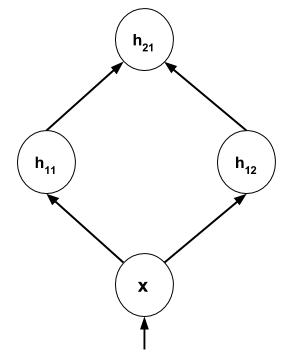
\includegraphics[scale=0.35]{sig2d}
          		  \end{center}
                  Plot the following functions: $h_{11}(x)$, $h_{12}(x)$ and $h_{21}(x)$ for $x \in (-1, 1)$
            \begin{solution}
            \vspace*{20mm}
            \end{solution}

            \part Now consider the variables $x_1, x_2$ and the functions $h_{11}(x_1, x_2), h_{12}(x_1, x_2), h_{13}(x_1, x_2), h_{14}(x_1, x_2)$, $h_{21}(x_1, x_2), h_{22}(x_1, x_2), h_{31}(x_1, x_2)$ and $f(x_1, x_2)$ such that   
   
                  \begin{align*}
                    h_{11}(x_1, x_2) &= \frac{1}{1 + e^{-(x_1 + 50x_2 + 100)}}  \\
                    h_{12}(x_1, x_2) &= \frac{1}{1 + e^{-(x_1 + 50x_2 - 100)}}  \\
                    h_{13}(x_1, x_2) &= \frac{1}{1 + e^{-(50x_1 + x_2 + 100)}}  \\
                    h_{14}(x_1, x_2) &= \frac{1}{1 + e^{-(50x_1 + x_2 - 100)}}  \\
                    h_{21}(x_1, x_2) &= h_{11}(x_1, x_2) - h_{12}(x_1, x_2)\\
                    h_{22}(x_1, x_2) &= h_{13}(x_1, x_2) - h_{14}(x_1, x_2)\\
                    h_{31}(x_1, x_2) &= h_{21}(x_1, x_2) + h_{22}(x_1, x_2)\\
                    f(x_1, x_2) &= \frac{1}{1 + e^{-(100h_{31}(x) - 200)}}  \\\\
                  \end{align*}
                  The above set of functions are summarized in the graph below.
                    \begin{center}
            		  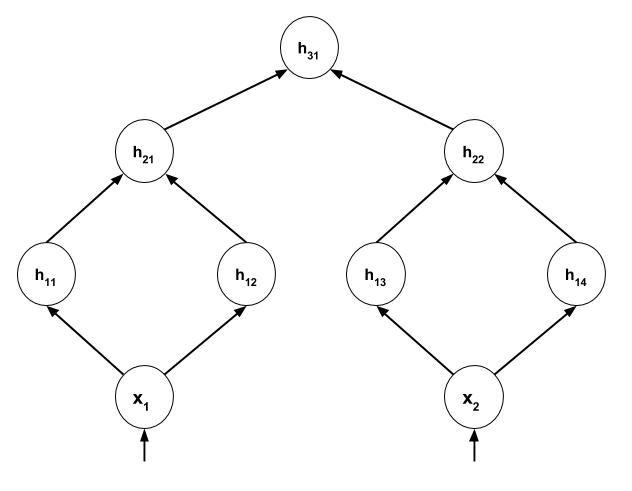
\includegraphics[scale=0.35]{sig3d}
          		    \end{center} 
                  Plot the following functions: $h_{11}(x_1, x_2), h_{12}(x_1, x_2), h_{13}(x_1, x_2), h_{14}(x_1, x_2), h_{21}(x_1, x_2),$ $h_{22}(x_1, x_2), h_{31}(x_1, x_2)$ and $f(x_1, x_2)$ for $x_1 \in (-5, 5)$ and $x_2 \in (-5, 5)$
            \begin{solution}
            \vspace*{20mm}
            \end{solution}
                 
           \end{parts}
\end{questions}             
\end{document}
